\begin{figure}[ht]
\centering

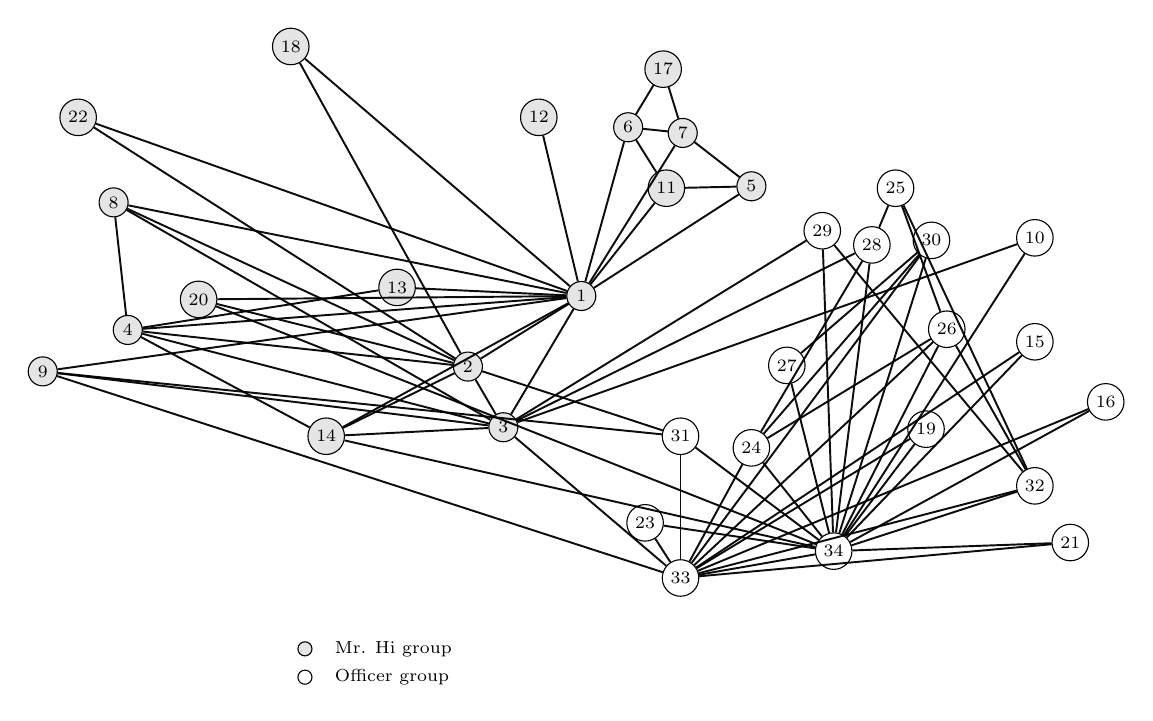
\begin{tikzpicture}[
  xscale=0.9, yscale=0.9, transform shape,
  hi/.style={circle, draw=black, fill=gray!20, inner sep=2.0pt, font=\scriptsize},
  off/.style={circle, draw=black, fill=white,   inner sep=2.0pt, font=\scriptsize},
  e/.style={line width=0.7pt, draw=black, opacity=0.95}
]

% (x and y stretched; coordinates updated directly)
\coordinate (p1) at (4.6,4.479);
\coordinate (p2) at (3,3.483);
\coordinate (p3) at (3.5,2.627);
\coordinate (p4) at (-1.8,4);
\coordinate (p5) at (7,6.027);
\coordinate (p6) at (5.261,6.860);
\coordinate (p7) at (6.031,6.780);
\coordinate (p8) at (-2,5.8);
\coordinate (p9) at (-3,3.415);
\coordinate (p10) at (11,5.3);
\coordinate (p11) at (5.8,6);
\coordinate (p12) at (4,7);
\coordinate (p13) at (2,4.6);
\coordinate (p14) at (1,2.5);
\coordinate (p15) at (11,3.833);
\coordinate (p16) at (12,2.985);
\coordinate (p17) at (5.755,7.680);
\coordinate (p18) at (0.5,8);
\coordinate (p19) at (9.464,2.6);
\coordinate (p20) at (-0.8,4.431);
\coordinate (p21) at (11.5,1);
\coordinate (p22) at (-2.5,7);
\coordinate (p23) at (5.5,1.278);
\coordinate (p24) at (7,2.336);
\coordinate (p25) at (9.034,6);
\coordinate (p26) at (9.757,4.010);
\coordinate (p27) at (7.5,3.5);
\coordinate (p28) at (8.7,5.2);
\coordinate (p29) at (8,5.4);
\coordinate (p30) at (9.541,5.264);
\coordinate (p31) at (6,2.5);
\coordinate (p32) at (11,1.8);
\coordinate (p33) at (6,0.500);
\coordinate (p34) at (8.161,0.879);



% --- Nodes (Mr. Hi vs Officer) ---
% Mr. Hi club: 1,2,3,4,5,6,7,8,9,11,12,13,14,17,18,20,22
\node[hi]  (p1)  at (p1)  {1};
\node[hi]  (p2)  at (p2)  {2};
\node[hi]  (p3)  at (p3)  {3};
\node[hi]  (p4)  at (p4)  {4};
\node[hi]  (p5)  at (p5)  {5};
\node[hi]  (p6)  at (p6)  {6};
\node[hi]  (p7)  at (p7)  {7};
\node[hi]  (p8)  at (p8)  {8};
\node[hi]  (p9)  at (p9)  {9};
\node[off] (p10) at (p10) {10};
\node[hi]  (p11) at (p11) {11};
\node[hi]  (p12) at (p12) {12};
\node[hi]  (p13) at (p13) {13};
\node[hi]  (p14) at (p14) {14};
\node[off] (p15) at (p15) {15};
\node[off] (p16) at (p16) {16};
\node[hi]  (p17) at (p17) {17};
\node[hi]  (p18) at (p18) {18};
\node[off] (p19) at (p19) {19};
\node[hi]  (p20) at (p20) {20};
\node[off] (p21) at (p21) {21};
\node[hi]  (p22) at (p22) {22};
\node[off] (p23) at (p23) {23};
\node[off] (p24) at (p24) {24};
\node[off] (p25) at (p25) {25};
\node[off] (p26) at (p26) {26};
\node[off] (p27) at (p27) {27};
\node[off] (p28) at (p28) {28};
\node[off] (p29) at (p29) {29};
\node[off] (p30) at (p30) {30};
\node[off] (p31) at (p31) {31};
\node[off] (p32) at (p32) {32};
\node[off] (p33) at (p33) {33};
\node[off] (p34) at (p34) {34};

% --- Edges (undirected) ---
\path[e] (p1) -- (p2);
\path[e] (p1) -- (p3);
\path[e] (p1) -- (p4);
\path[e] (p1) -- (p5);
\path[e] (p1) -- (p6);
\path[e] (p1) -- (p7);
\path[e] (p1) -- (p8);
\path[e] (p1) -- (p9);
\path[e] (p1) -- (p11);
\path[e] (p1) -- (p12);
\path[e] (p1) -- (p13);
\path[e] (p1) -- (p14);
\path[e] (p1) -- (p18);
\path[e] (p1) -- (p20);
\path[e] (p1) -- (p22);
\path[e] (p2) -- (p3);
\path[e] (p2) -- (p4);
\path[e] (p2) -- (p8);
\path[e] (p2) -- (p14);
\path[e] (p2) -- (p18);
\path[e] (p2) -- (p20);
\path[e] (p2) -- (p22);
\path[e] (p2) -- (p31);
\path[e] (p3) -- (p4);
\path[e] (p3) -- (p8);
\path[e] (p3) -- (p9);
\path[e] (p3) -- (p10);
\path[e] (p3) -- (p14);
\path[e] (p3) -- (p28);
\path[e] (p3) -- (p29);
\path[e] (p3) -- (p33);
\path[e] (p4) -- (p8);
\path[e] (p4) -- (p13);
\path[e] (p4) -- (p14);
\path[e] (p5) -- (p7);
\path[e] (p5) -- (p11);
\path[e] (p6) -- (p7);
\path[e] (p6) -- (p11);
\path[e] (p6) -- (p17);
\path[e] (p7) -- (p17);
\path[e] (p9) -- (p31);
\path[e] (p9) -- (p33);
\path[e] (p10) -- (p34);
\path[e] (p14) -- (p34);
\path[e] (p15) -- (p33);
\path[e] (p15) -- (p34);
\path[e] (p16) -- (p33);
\path[e] (p16) -- (p34);
\path[e] (p19) -- (p33);
\path[e] (p19) -- (p34);
\path[e] (p20) -- (p34);
\path[e] (p21) -- (p33);
\path[e] (p21) -- (p34);
\path[e] (p23) -- (p33);
\path[e] (p23) -- (p34);
\path[e] (p24) -- (p26);
\path[e] (p24) -- (p28);
\path[e] (p24) -- (p30);
\path[e] (p24) -- (p33);
\path[e] (p24) -- (p34);
\path[e] (p25) -- (p26);
\path[e] (p25) -- (p28);
\path[e] (p25) -- (p32);
\path[e] (p26) -- (p32);
\path[e] (p26) -- (p33);
\path[e] (p26) -- (p34);
\path[e] (p27) -- (p30);
\path[e] (p27) -- (p34);
\path[e] (p28) -- (p34);
\path[e] (p29) -- (p32);
\path[e] (p29) -- (p34);
\path[e] (p30) -- (p33);
\path[e] (p30) -- (p34);
\path[e] (p31) -- (p33);
\path[e] (p31) -- (p34);
\path[e] (p32) -- (p33);
\path[e] (p32) -- (p34);
\path[e] (p33) -- (p34);

% (named nodes already declared earlier)

% --- Small legend ---
\node[hi]  at (0.7,-0.5) {};
\node[draw=none, font=\scriptsize, anchor=west] at (1.0,-0.5) {Mr. Hi group};
\node[off] at (0.7,-0.9) {};
\node[draw=none, font=\scriptsize, anchor=west] at (1.0,-0.9) {Officer group};

\end{tikzpicture}
\caption{A social network of 34 members divided into two groups: Mr. Hi and Officer. Edges represent friendships between members.}  
\end{figure}